\documentclass[letterpaper,12pt]{cicese}
	\usepackage[letterpaper,left=2.5cm,right=2.5cm,top=3cm,bottom=3cm]{geometry}
	\usepackage{setspace}
	\usepackage{natbib}
	\usepackage{graphicx}
	\usepackage{float}
	\usepackage{caption}
	\begin{document}
	\doublespace
	\title{Detecci\'on de Estr\'es Por Medio de C\'omputo Vestible}
	\author{Dari\'en Alberto Miranda Boj\'orquez}
	\maketitle
	\newpage
	\tableofcontents
	\newpage

		\chapter{Introducci\'on} 
			El estr\'es es un fen\'omeno que la poblaci\'on de nuestra sociedad moderna experimenta cotidianamente. S\'olo en Estados Unidos, tres cuartos de sus
			habitantes experimentan s\'intomas relacionados con el estr\'es \citep{Lu2012}. El estr\'es se demuestra de diferentes maneras en las personas tanto psicol\'ogica
			como fisiol\'ogicamente. Los efectos psicol\'ogicos incluyen: ansiedad, depresi\'on, desgaste, insomnio e insatisfacci\'on \citep{Sebastian2013556}. La relaci\'on que tiene
			con la ansiedad es que la ansiedad es la se\~nal psicofisiol\'ogica de que la respuesta al estr\'es ha sido iniciada.\citep{PMID2235645}
			
			
			Un cierto  nivel de estr\'es es necesario para lograr las tareas de los trabajos de nuestra sociedad moderna. Nos impulsa a completar tareas basadas en 
			calendarios. Incluso, \emph{``El estr\'es puede no ser observado como un problema por las personas, niveles altos de estr\'es  son percibidos com\'unmente 
			como una norma, una se\~nal de que est\'an  haciendo su mejor esfuerzo para completar objetivos"}\citep{Bakker2012SMS}. Durante una situaci\'on de estr\'es, el cuerpo se encuentra
			tensando los m\'usculos mientras que el sistema nervioso parasim\'etrico trabaja para controlar este problema balanceandolos para lograr una homeostasis\citep{Ayzenberg2012}. Sin
			embargo, periodos largos en este estado pueden llevar a problemas de salud como dolores de cabeza, fatiga, ansiedad y depresi\'on.
			%como puede llegar a ser un desorden? (post traumatic disorder)
			%computo vestible

			Por otro lado, el c\'omputo vestible nos permite llevar computadoras con nosotros de la misma manera que llevamos la ropa puesta. Al "vestir" un dispositivo,
			el usuario tiene acceso a una computadora que es capaz de hacer monitor de \'el mismo as\'i de su entorno por medio de sensores. Dichos sensores pueden medir entre
			otras cosas: movimientos del cuerpo del usuario, la posici\'on del usuario, intensidad de luz, ruido, im\'agenes de su ambiente, ritmo card\'iaco, capacidad
			conductiva de la piel, distancias, entre otros. Debido a su caracter\'istica de ser vestible, se pueden hacer monitoreos constantes y mas precisos que con
			los sistemas tradicionales, adem\'as de ayudar en las tareas de la vida cotidiana en las que el c\'omputo tradicional de escritorio no puede alcanzar.
			
			El uso de c\'omputo vestible para la detecci\'on de el estr\'es abre una posibilidad para ayudar en las tareas cotidianas y reducir el riesgo a la salud mental
			del usuario que el estr\'es asociado.
		\chapter{Marco te\'orico} 
			A continuaci\'on, se definen los conceptos al rededeor de la naturaleza y detecci\'on del estr\'es. Los aspectos tecnol\'ogicos y psicol\'ogicos son explicados.
			%stimuli
			\section{Estr\'es}
				El estr\'es puede ser visto como una carga mental o \emph{stimuli} el cual tiene un peso asociado. Este peso puede ser positivo o negativo dependiendo
				de la apreciaci\'on del sujeto. Cuando percibimos un \emph{stimulus} o un grupo de {stimuli} como amenzante, lo especificamos como \emph{estr\'es}\citep{Sebastian2013556}.
				Este es un tipo de experiencia que puede ser f\'acilmente cuantificada por medio de instrumentos psicol\'ogicos.
				
				El modelo descrito por Levine \citep{Sebastian2013556} explica el proceso del estr\'es de la siguiente manera: La carga, que incluye los factores estresantes y el
				stimuli es evaluada por el cerebro. Despu\'es de la evaluaci\'on, puede haber una respuesta al estr\'es, la cual funciona como alarma para el cerebro.
				El cerebro puede entonces modificar el stimuli o la percepci\'on del stimuli por medio de acciones y periodos de inactividad. Por \'ultimo, la respuesta
				fisiol\'ogica puede generar tensi\'on  o entrenamiento, dependiendo de la actividad. Un estr\'es sostenido puede llevar a una patolog\'ia (tensi\'on).
			\section{Caracterizaci\'on fisiol\'ogica}
				Los m\'etodos comunes para la detecci\'on del estr\'es por medio de se\~nales fisiol\'ogicas son: 
					\begin{itemize}
						\item \emph{Frecuencia Card\'iaca (HR).} Normalmente, suponen que el ritmo card\'iaco aumenta durante los periodos de estr\'es. 
						\item \emph{Respuesta Galv\'anica de la piel (GBR).} De la misma manera que el ritmo card\'iaco, la respuesta galv\'anica de la piel suele cambiar durante los periodos de estr\'es.
						\item \emph{Procesamiento del lenguaje natural.} Algunas sutilezas del habla suelen notarse en los periodos de estr\'es, tales como tartamudeo o tonos de voz.
						El procesamiento del lenguaje natural puede ser utilizado como herramienta de medici\'on de estr\'es.
					\end{itemize}
			\section{C\'omputo vestible}
				El c\'omputo vestible es aquel en el que la computadora es lo suficientemente peque\~na para poder ser "vestida" como ropa mientras que asiste en las
				tareas cotidianas de la vida del usuario\citep{Starner97augmentedreality}. Algunos lugares t\'ipicos del cuerpo donde son usados son: los ojos, o\'idos, brazos, piernas o torso.
				Los individuos que usan estos dispositivos suel cargarlos f\'acilmente con ellos por largos periodos de tiempo durante el d\'ia. Al tener sensores
				especializados, y si consideramos que el usuario puede llevar mas de uno puesto, tenemos una herramienta de sensado poderosa que es capaz de obtener
				informaci\'on del cuerpo del individuo al mismo tiempo que provee una comunicaci\'on mas natural que aquella del c\'omputo tradicional del escritorio.

			\section{Contexto}
				El contexto es definido por Dey \citep{Dey2001} como toda aquella informaci\'on que puede ser utilizada para caracterizar la situaci\'on de una entidad. Donde una
				entidad puede ser una persona, lugar u objeto computacional. El tener informaci\'on contextual permite a los programas funcionar de una manera adaptativa,
				en la que toma en cuenta la situaci\'on y act\'ua acorde a ella. Un ejemplo de c\'omputo contextual que usamos diaramente es el tel\'efono inteligente.
				Si el ambiente del usuario tiene mucha luz, el tel\'efono decide reducir el brillo de la pantalla, o bien, si se est\'a haciendo una llamada en un lugar muy ruidoso,
				decide aplicar filtros de ruido para mejorar la calidad de la voz.
		
			\section{C\'omputo vestible consciente del contexto}
				Al encontrarse cerca del usuario mientras ayuda en las tareas diarias, el c\'omputo vestible debe de hacer uso del contexto para ayudar de una manera
				que sea significante para el usuario. De no ser as\'i, puede generar frustraci\'on y desuso. Algunas de las caracter\'isticas del c\'omputo vestible
				con respecto al contexto que deben de tener estos dispositivos seg\'un \citep{Rhodes97thewearable} son las siguientes:
				\begin{itemize}
					\item{\emph{Port\'atil y al mismo tiempo operacional:}} Una computadora vestible es capaz de ser usada mientras que el usuario se encuentra
					en movimiento. Al estar en movimiento, su contexto es much mas din\'amico: Cambia a nuevos espacios f\'isicos, encuentra nuevos objetos 
					y gente (entidades).Los servicios e informaci\'on que requiere cambiar\'an en base a las nuevas entidades.
				\end{itemize}
				\begin{itemize}
					\item{\emph{Uso en modo manos libres:}} Una computadora vestible tiene la intenc\'ion de ser operada con m\'inimo uso de las manos,
					bas\'andose en la entrada por voz o controles con una sola mano. Limitar el uso de los mecanismos de entrada incrementa la necesidad
					de obtener informaci\'on contextual impl\'icitamente sensada.
				\end{itemize}
				\begin{itemize}
					\item{\emph{Sensores:}} Para disminuir la entrada expl\'icita del usuario, una computadora vestible deber\'ia de utilizar sensores para
					colectar informaci\'on acerca del ambiente del usuario. La informaci\'on obtenida directamente por los sensores en el cuerpo del
					usuario puede ser combinada con sensonres puestos en el ambiente en aplicaciones reales.
				\end{itemize}
				\begin{itemize}
					\item{\emph{Pro activo:}} Una computadora vestible debe de actuar en base al comportamiento del usuario incluso cuando el usuario no
					est\'a expl\'icitamente utiliz\'andolo. Esta es le esencia de la computaci\'on basada en el contexto: la computadora analiza el
					contexto de usuario y provee de tareas y servicios relevantes a las actividades del usuario interrumpiendolo s\'olo cuando es apropiado.
				\end{itemize}
				\begin{itemize}
					\item{\emph{Siempre encendido:}} Una computadora vestible siempre est\'a encendida. Esto es importante para el c\'omputo consciente del contexto
					porque la computadora vestible debe de monitorear constantemente la situaci\'on del usuario para que se pueda adaptar y responder
					adecuadamente. Debe de ser capaz de proveer servicios \'utiles al usuario en cualquier momento.
				\end{itemize}
				%como se usa todo esto para dar soporte a las actividades de la vida diaria?

		\chapter{Trabajo previo}
				Diferentes trabajos se han realizado para la detecci\'on del estr\'es. A continuaci\'on se listan algunos de los mas relevantes:
				\begin{itemize}
					\item{\emph{AutoSense}\citep{Ertin2011}} es un dispositivo especialmente dise\~nado para el sensado del estado del estr\'es del usuario. Posee seis diferentes
					sensores que pueden colectar informaci\'on cardiovascular, respiratoria, t\'ermica, de respuesta galv\'anica de la piel y de acelerometr\'ia. Los
					datos son luego enviados por medio de una conexi\'on bluetooth a una aplicaci\'on en Android donde se realizan inferencias y provee una capa de 
					servicio a otras aplicaciones.
		
					\item{\emph{FaceIt}\citep{Rennert2013}} es una herramienta que permite detectar, almacenar y recordar situaciones en las que el usuario presente ansiedad. Utiliza
					de base la Terapia de Comportamiento Cognitiva (CBT por sus siglas en ingl\'es). Un dispositivo vestible tipo Memoto que cuelga del cuello del usuario
					detecta por medio del ritmo card\'iaco los episodios de ansiedad y registrs solo en esos momentos video, audio y la localizaci\'on geogr\'afica. Posteriormente,
					los datos son transmitidos a internet, y una p\'agina web les permite a los pacientes almacenar sus periodos y revivir las situaciones de manera
					controlada. En este estudio indican que \emph{``Los dispositivos m\'oviles ya se han vuelto parte de nuestra vida diaria. Otras tecnolog\'ias vestibles 					se est\'an volviendo comunes"}. La investigaci\'on tambi\'en indica que: \emph{``las aplicaciones m\'oviles tienen la capacidad de incrementar
					la autoconciencia y reducir los niveles de estr\'es"}.  que \emph{``Por estas razones, creemos que este enfoque tiene el potencial de asisistir
					el tratamiento de comportamiento cognitivo para aquellos con ansiedad social"}.

					\item{\emph{Stress@work}\citep{Bakker2012SMS}} es un marco de trabajo para la medici\'on, entendimiento y predicci\'on y manejo del estr\'es. Utiliza la Respuesta
					Galv\'anica de la piel y los eventos calendarizados en Microsoft Outlook para inferir y predecir periodos de estr\'es. Al detectar los periodos de
					carga de estr\'es, da recomendaciones de recalendarizaci\'on de actividades para balancear dichas cargas.
				\end{itemize}
		\chapter{Objetivos}
			\section{General}
				\begin{enumerate}
					\item Encontrar de que manera los dispositivos vestibles pueden ayudar a detectar periodos de estr\'es.
				\end{enumerate}
			\section{Espec\'ificos}
				\begin{enumerate}
					\item Encontrar que informaci\'on contextual es la m\'as adecuada para detectar periodos de estr\'es.
					\item Desarrollar un modelo matem\'atico para la detecci\'on de estr\'es.
					\item Encontrar que dispositivos vestibles son los mas adecuados para recolectar la informaci\'on para detectar periodos de estr\'es.
					\item Desarrollar un prototipo de detecci\'on de periodos de estr\'es.
					\item Evaluar el prototipo.
				\end{enumerate}
			\section{Preguntas de investigac\'ion}
				\begin{enumerate}
					\item >C\'omo pueden los dispositivos vestibles ayudar a detectar periodos de estr\'es?
				\end{enumerate}
		\chapter{Metodolog\'ia}
				\begin{enumerate}
					\item Revisi\'on de la literatura.
					\item Selecci\'on de escenario de estudio.
					\item Identificaci\'on de los tipos de se\~nales mas significativas para medir el estr\'es en el escenario seleccionado.
					\item Revisi\'on y selecci\'on de los dispositivos vestibles disponibles en el mercado para los tipos de datos seleccionados.
					\item Desarrollo de soluci\'on de software.
					\item Validaci\'on del software por medio de experimentaci\'on.
					\item Presentaci\'on de resultados.
				\end{enumerate}
		\chapter{Importancia de la investigaci\'on}
				Una de las finalidades de la tecnlog\'ia es ayudar en los problemas de los humanos. Los avances recientes en c\'omputo vestible muestran
				ser una poderosa herramienta para monitorear nuestros cuerpos, debido a que son f\'aciles de vestir, cuentan con diversos sensores y se pueden
				llevar con nosotros una buen parte del d\'ia. Ese monitoreo constante es \'util tambi\'en para mejorar la calidad de vida en personas con alta
				carga de estr\'es. A continuaci\'on se describen posibles escenarios de aplicaciones reales.
				
				\section{Escenarios de aplicaci\'on}
				\begin{enumerate}
					\item \emph{Cuidadores de autismo.}
					El desorden de autismo ( referido como autismo ) es una de las variedades del Espectro de Des\'ordenes del Autismo (ASD) y est\'a caracterizado por
					interacciones sociales da\~nadas, ausencia de habilidades de comunicaci\'on, movimientos estereotipados y mal comportamiento en general\citep{bernier2010autism}. Existen
					escuelas especiales para ni\~nos con este padecimiento. Mar\'ia es una maestra novata de este tipo de escuelas. Entre sus labaores, se encuentra
					atender a un grupo de mas de diez alumnos. Tratar con los ni\~nos es una labor muy exigente y estresante. Si Mar\'ia llega al l\'imite de su capacidad
					de carga de tareas, su calidad como maestra y su estado de salud puede verse disminu\'ido temporalmente. Juliana, la encargada del personal de la
					escuela debe ser capaz de saber si Mar\'ia est\'a siendo afectada severamente y pasar la carga a otra maestra mas desocupada o bien, con mas experiencia. Mar\'ia
					tiene un dispositivo vestible que incluye sensores que infieren el estado de estr\'es en ella y que adem\'as registra por medio de video y su
					frecuencia card\'iaca los eventos de estr\'es. El dispositivo indica a Juliana el nivel de estr\'es y le permite hacer el cambio de maestra. Luego,
					en una reuni\'on, Juliana utiliza los videos de los eventos de estr\'es para ayudarle a Mar\'ia a controlarlos y ganar experiencia.
					\item \emph{Cuidadores de Pacientes con demencia.}
						La demencia es un s\'indrome del declive de las habilidades cognitivas. Los s\'intomas comunes son: problemas de memoria, dificultades para
						realizar tareas familiares, mal juicio, deterioro del lenguaje hablado y cambios de humor\citep{Aziz}. Afecta alrededor del 4\% de las personas
						mayores de 65 a\~nos y al 40\% de las personas mayores de 90. Valeria tiene un padre con demencia. Le toma una buena parte del d\'ia ayudarlo
						con tareas cotidianas como ayudarle a lavarse los dientes, cambiarse, recordarle donde puso los lentes, proporcionarle sus medicinas entre
						otras tareas. Adem\'as de cuidarlo, Valeria tiene un trabajo de medio tiempo como oficinista y es madre de dos hijos en escuela primaria.
						El constante cambio de roles y su poca experiencia como cuidadora, le genera una alta cantidad de estr\'es, y le es dif\'icil manejar sus
						propias necesidades. Sufre de lapsos donde su ritmo card\'iaco y de respiraci\'on se encuentran muy alterados y no le permite pensar
						claramente. Un dispositivo vestible que detecta los episodios de estr\'es, le da recomendaciones sobre como tranquilizarse a trav\'es de
						sencillos ejercicios de respiraci\'on.
					\item \emph{Administrador de proyectos.}
						Sebasti\'an es un administrador de proyectos en una empresa de software. Entre sus tareas, se encuentra asegurarse que diferentes proyectos
						se ejecuten al tiempo correcto. Si una tarea de un proyecto se encuentra retrasada, es su responsabilidad contactar al jefe responsable.
						Tambi\'en se encarga de realizar reuniones con los equipos de trabajo para escuchar sus problemas y peticiones. Estas reuniones suelen
						alargarse en tiempo y los conflictos entre los equipos suelen ser graves. El disposito que viste Sebasti\'an le permite conocer en que
						reuniones y en que tiempos del desarrollo del proyecto se presentan diferentes \'indices de estr\'es. Una agenda inteligente le permite
						distribuir las cargas de estr\'es durante la semana para evitar riesgos de salud.
				\end{enumerate}
		\chapter{Limitaciones y suposiciones}
			Se tomar\'an en cuenta solamente la detecci\'on de estr\'es bajo ciertos escenarios, debido a que las situaciones en las que una persona puede sufrir estr\'es son muy variadas como para englobarlas en una sola soluci\'on tecnol\'ogica.
			La naturaleza de esta investigaci\'on requiere de dispositivos con sensores especializados como medidores de frecuencia cardi\'aca y resistencia galv\'anica de la pielentre otros. A pesar de que la tecnolog\'ia m\'ovil y vestible ha logrado una importante penetreaci\'on en el mercado, la l\'inea base de dispositivos no cuenta con dichos sensores. Al requerirse esta particularidad en los dispositivos, podr\'ian desprenderse subtareas como el contacto con empresas especializadas, espera de entrega, y entrenamiento en el desarrollo para estas tecnolog\'ias. Dichas tareas podr\'ian tomar un tiempo considerable en el proceso de investigaci\'on. Debido a esto, ser\'a importante organizar los tiempos muertos para evitar retrasos en la finalizaci\'on del estudio.
			Por otro lado, el uso de dispositivos que a\'un no ingresan al mercado t\'ipico mexicano podr\'i no representar el uso cotidiano del que la visi\'on del  c\'omputo ubicuo habla. Sin embargo, buscar\'an estrategias para combinar y adaptar la tecnolog\'ia disponible para lograr una situaci\'on mas realista.
		\chapter{Contribuci\'on al conocimiento}
			El desarrollo de esta investgiaci\'on contribuir\'a a la interacci\'on humano computadora en forma de modelos matem\'aticos y/o estad\'isticos que permitan la inferencia de estr\'es utilizando dispositivos vestibles. As\'i de como recomendaciones para el dise\~no de aplicaciones futuras que utilicen estos modelos.
		\chapter{Calendario de actividades}
			
		\begin{figure}
		  \begin{center}
		  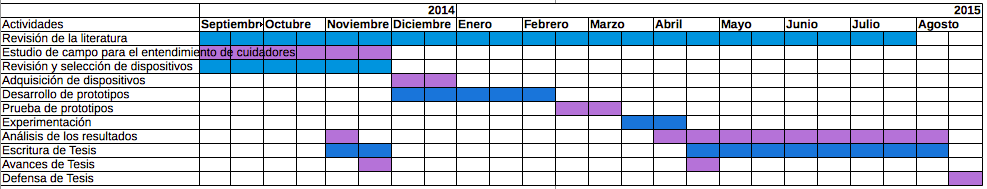
\includegraphics[]{cal}
		  \end{center}
		\end{figure}
	%1 StressSense: detecting Stress in Unconstraner Acoustic Environments using smartphones
	%2 A thoerical approach to stress and self-efficacy
	%3 Stress and anxiety, 	Department of Psychophysiological Nursing, School of Nursing, University of Maryland, Baltimore.The Nursing Clinics of North America [1990, 25(4):935-943]
	%4 AutoSense: Unobtrusively Wearable Sensor Suite for Inferring the Onset, Causality, and Consequences of Stress in the Field
	%5
	%6 stress@work
	%7 FEEL: frequent EDA and Event Logging
	\addcontentsline{toc}{chapter}{\normalsize\expandafter{Referencias}}
{\normalsize
\bibliographystyle{cicese}
\bibliography{referencias}
}
	\end{document}
